\message{ !name(Orpheus_ISGT-EUR.tex)}%% started from bare_conf.tex template.

\documentclass[conference]{IEEEtran}
\usepackage{graphicx}
\usepackage[cmex10]{amsmath}
%\usepackage{algorithmic} 
\usepackage{array} %TBD
\usepackage{subfigure} %TBD
\usepackage{url} 

% correct bad hyphenation here
%\hyphenation{op-tical net-works semi-conduc-tor}

\begin{document}

\message{ !name(Orpheus_ISGT-EUR.tex) !offset(-3) }


% paper title
\title{(TBD) Optimizing Hybrid Energy Grids for Smart Cities: an
  Investigation Platform} 
% investigation? platform? process? "Investigating impact of Hybrid?"
% "Investigating Optimization of Hybrid Energy Grids for Smart Cities:
% [some more words?]"

% author names and affiliations
\author{\IEEEauthorblockN{Tae-Gil Noh, S\'ebastien Nicolas, \\ Maja
    Schwartz and Anett Sch\"ulke}
\IEEEauthorblockA{NEC Laboratories Europe\\
Heidelberg, Germany\\
\{tae-gil.noh, sebastien.nicolas,\\maja.schwarz, anett.schuelke\}@neclab.eu}
\and
\IEEEauthorblockN{Daniel Schwaweneder and Hans Auer}
\IEEEauthorblockA{Inst. of Energy Systems and Electrical Drives\\
  Vienna University of Technology\\
Vienna, Austria\\
\{schwabeneder, auer\}@eeg.tuwien.ac.at}
}

% make the title area
\maketitle

% As a general rule, do not put math, special symbols or citations
% in the abstract
\begin{abstract}
The abstract goes here. (limited to 150 words). 
% Words written to check
% the size of 150 words. Words written to check the size of 150 words.  
% Words written to check the size of 150 words.  Words written to check
% the size of 150 words.  Words written to check the size of 150 words.
% Words written to check the size of 150 words.  Words written to check
% the size of 150 words.  Words written to check the size of 150 words.
% Words written to check the size of 150 words.  Words written to check
% the size of 150 words.  Words written to check the size of 150 words.
% Words written to check the size of 150 words.  Words written to check
% the size of 150 words.  (125 words) 
\end{abstract}

% no keywords
% (GIL) TODO: put keywords, before make it final. 
\begin{IEEEkeywords}
keyword1, keyword2, keyword3 
\end{IEEEkeywords} 

\IEEEpeerreviewmaketitle

%%%
%%%
%%% start of the manuscript 

\section{Introduction}
% First two paragraphs are borrowed from D5.1 and 
% *heavily* revised. -- still don't like them but ... 
The electricity grid model is evolving from a hierarchic 
centralized architecture towards a decentralized one. 
One of the main challenge in this course for future energy grid is the  
lack of flexibility to integrate high penetrations of volatile
renewable energy sources in the existing power grids. 
The challenge is about how a temporary energy surplus at one time can
be managed. It can either saved for the grid at low-generation times
(e.g. storage), or utilized more efficiently in time- and
location-effective manner (e.g. local consumption, local
transformation). 
Hybrid energy networks can be regarded as one of the opportunities to  
provide solutions for managing this imbalance \cite{appelrath_2012}.  
% ideally? in Ideal form, 
A hybrid energy network is an energy system operated across different 
domains (such as over Gas, district heat, and power grids) whereby
energy will be transformed between the grids. In this network, the
energy can be consumed, stored, transported with a grid in its
specific form or to be transformed into other energy form between
different grids, for different times and/or locations.
The advantages of such an approach are the increase in reliability,
flexibility and the synergy effect \cite{arnold_2011}. 

The development of smart grids on each energy grid, independently,
has been progressed and supported with extensive research for many
years. One prominent next step in the energy network evolution path
will be the connection and integration of different energy grids
(multiple carrier grids) – realizing Hybrid Energy Networks
efficiently operated through coupling points (e.g. CHP and
power to gas plants) and managed cooperatively. The energy operators
can take advantage of the characteristics of each energy carrier and
exploit, for example, the possibility of transmitting energy as
electricity and storing energy as gas and as warm water in
accumulators. 
% TODO, check better citations (with Daniel) 
Investigation of this hybrid evolution path is still in
its infancy. There has been some investigation of individual
components \cite{keirstead_2012}, or possible control strategies
\cite{arnold_2009}, but they generally lack the full investigation on
their impact of hybridization in real-world environment. A thorough 
investigation, which includes all major stake-holders in place that
are modeled from real-world cities, will open more convincing and
exciting new possibilities for future energy grids.   

In this paper, we introduce an investigation platform that is designed  
to develop and evaluate novel co-operative, co-existing hybrid grid
control strategies. The process starts with a set of hybridization
setups identified from two European cities. The setups represents
hybridization chances that we have spotted from the target sites. 
By adding specific technological and economical goals of the 
stake-holders to the setups, we identify concrete hybridization
scenarios. Then, for each identified scenario, we go through 
two-step investigation process based on co-simulation and
economical-model. The simulation investigation focuses on
technological and operational observations, while the economical model
measures socio-economical impacts in the long-term.  
The target of this holistic investigation is to understand the
range of flexibility given through the coupling of energy grids. 
% to understand which level and which quality of ICT,
%sensor/monitoring and automatic control technologies are required to
%realize the distributed system intelligence.  
% We believe that the proposed platform enables us to investigate not
% only the technical impacts, but also social-/economical aspects to
% identify future evolutionary path for energy grids.  
We believe that the proposed platform enables us to fully investigate
this flexibility, which will result concrete recommendations for
future evolution of energy grids. 

% The paper proceeds as follows: Section \ref{sec:soa} summarizes
% current states and related work, and Section \ref{sec:req}
% introduces the identified hybrid setups and requirements of the
% investigation. Section \ref{sec:econ} shows the economical model being
% employed within the investigation, and Section \ref{sec:hol} shows the
% holistic investigation steps. Finally, Section \ref{sec:con}
% introduces outlook of the expected results and concludes. 

\section{State of the art}
\label{sec:soa}
%The increasing energy demand as well as the increasing fluctuating
%energy production from renewable energy sources (RES) such as wind and
%solar power are posing a major challenge for European energy
%networks. This is especially true for electricity transmission and
%distribution grids. They 
Electricity networks have been mostly constructed before the
liberalization of the European energy markets and were designed for
unidirectional load flows from large generation plants to the end
users. With the unbundling of the energy supply chain, technological
advancements of renewables, support mechanisms to promote their
installation, increasing environmental awareness and more active
participation of customers, the amount of distributed (small-scale)
generation plants and de-centralized feed-in of electricity has
considerably increased in recent years. Thus, energy distribution
system operators (DSO) have to cope with bidirectional load flows in
their networks and both, DSOs and energy supply companies, have to
deal with decreasing turnover. Furthermore, fluctuating energy
production from renewable energy sources (RES) - from large-scale to
household level - is de-coupled from  energy demand, which is 
causing a lack of storage in the electricity network.

In general, this issue can be partially tackled by (i) shedding
renewables during hours of high production, (ii) increasing
transmission capacity of the electricity network, (iii) installing
additional capacities of energy storages and/or (iv) increasing the
flexibility of demand. The first option is neither desirable from an
economic, nor from an environmental point-of-view. However, nowadays
this is often the only possibility available. The second alternative
is very costly, currently subject to many political and public
discussions and might be necessary anyway. However, it probably will
not be a sufficient solution on its own. The economic potential of
electric energy storages is limited due to the high investment cost
and the phenomenon of economic cannibalism of storages: The
profitability of electric storages depends on the spread of
electricity prices (at least in the current market design) and, at
the same time, increasing storage capacity
is reducing this spread. Regarding the flexibility of demand, many
smart grid projects related to demand response, virtual power plants
and similar approaches are currently being implemented. However, the
potential on the electricity domain only is limited. 

Considering other energy domains and networks, like gas and district
heating, as well can significantly increase the storage capacity and
demand flexibility potentials. Conversely, these domains can benefit
from a closer interaction with the electricity domain too. Converting
electric energy when production from renewables is high and
electricity demand is low, for instance, can reduce the usage of
fossil fuels for heat production. Though these synergies are becoming
increasingly apparent, the full potential of cooperation among
different energy domains is not yet nearly exploited. There are
several reasons for this: For one thing, different energy domains are,
in fact, competing for the customers’ energy demand. Space heating
can, for instance, be provided by a district heating network, by a gas
network via residential gas boilers or by the electricity network
using e.g. a heat pump or an electric boiler. Thus, different market
participants (DSOs, supply companies) operating on different energy
domains are rather interested in maximizing their own turnover and
profit than in finding cooperative strategies to increase total
efficiency. Furthermore, there are some structural and regulatory
issues complicating a connection and cooperation between different
energy networks. It is possible, for instance, that using cheap excess
electricity from RES production for heating is not economical compared
to using other fuels due to electricity network charges, even though
an increased electricity demand could support network operation or
prevent shedding of renewables. Besides, network operators, who could
significantly benefit from increased flexibility via coupling
technologies for balancing, are not permitted to own, operate or
control energy storage or conversion devices in the current market
structure. 

In this paper a concept and methodology is presented, how different
hybrid cooperative control strategies can be developed, which aim to
increase the efficiency of hybrid energy networks. Special focus is
laid on exploiting the synergies among different energy domains and,
hence, increasing the flexibility of energy networks and facilitating
the integration of RES. Furthermore, this approach emphasizes a
multi-agent perspective by taking into account the individual
objectives of different market participants in a hybrid energy supply
chain aiming to develop cooperative strategies among competitors
resulting in win-win situations. Moreover, this concept will be used
to identify barriers in today’s regulations, hampering a closer
interaction among different energy domains, and go beyond current
market rules to examine possible future hybrid control strategies and
business models.


\section{Investigating Hybrid-grid Control Strategy: 
Setups and Requirements}
\label{sec:req}

% Assumption on problem / intro introduced: difficulty of Hybrid, and
% our main attack points: 
% \begin{itemize}
% \item  a) synth. data of sim (not realistic) $\Rightarrow$ actual
%   cities.  
% \item  b) requires both view of eco+tech (not just tech only)
%   $\Rightarrow$ dual investigation 
% \end{itemize}

\subsection{Identifying Hybrid Setups from the Two European Cities}
%% (Spotting hybrid setups from European cities?) 
\label{sec:req-1}
Our goal is to investigate the impact of {\em co-operative,
  co-existence control} over multiple energy grids of future cities, 
and understand the range of flexibility given through the coupling of
the energy grids. 
We start our investigation process by spotting possible hybrid chances 
from two European cities. Our two target sites are the city of
Skellete\aa, Sweden, and two small towns near Ulm, Germany.  

Skellefte\aa is a city of Sweden in mid-northern part with sub-arctic
climate. Population of the city is over 32,000, and served by district
heat (DH) grid with around 4200 heating substations. For a typical
year, the DH grid provides about 343,000 MWh of heat to the
city. Base heat load is being served by a CHP, which uses bio-mass
fuel to generate heat and power. The city also has traditional power
grid, and both grids are controlled by Skellefte\aa Kraft, which is
owned by the municipality. 
Town of Einsingen and Hittistetten are located in the suburb of Ulm, 
Germany. They are small residential towns with some commercial and
public spaces. They have registered population of 400 and 300
respectively. Both towns are characterized by relatively high-level of 
PV penetration: 21 panels and 233kWp in Einsingen, 58 panels and 
1.16MWp in Hittistetten. In addition to Power grid, the towns have
gas-grids that serves as the most common heating mean. There are also 
some houses with oil and electric boiler.  

With close support from Skellefte\aa Kraft and Stadtwerk Ulm, we have
identified three {\em hybrid control setups} , which forms the
starting point of hybrid-investigations.   
Table \ref{tab:1} summarizes the three setups. {\em Co-operative
  suppliers} is a hybrid setup that focuses on supplier side
hybridization. Here, the participants are energy providers and DSOs of 
power and DH grids. The means for hybridization (the exists and can be
added for better co-operative control) are devices that connect DH and 
Power grids on supplier side, such as CHP (as generation to both
grids), and e-boilers (power to heat grid). In this setup, the synergy
comes from operating both power and heat supply in co-operation. 
{\em Prosumer Community} focuses on consumer side. The participants of
this setup are consumer and DSO, where the consumer has renewable
energy (RES) generation capability. The hybrid nature of this setup
comes from consumers side, which participate multiple grids with
multiple devices. The hybrid synergy can be tapped by co-operative
control of using RES energy with house-hold heat demand (such as
domestic hot water). 
The final setup, {\em Interacting providers and consumers}, targets
both Ulm and Skellefte\aa. This setup aims further future situation on
both sites, such as introducing new grids or major changes. The
setup assumes tighter ICT connection of smart cities, which will
enable far higher (in time and data amount) interactions that were
previously not possible, not only between provider/consumer, but also
between energty grids and between consumer devices on different grids.   
%This setup also assumes long-term evolution such as
%adding new grids, or new regulations. 

% [we are trying to generalize, for future investigation] 
Each hybrid setup represent a class of hybridization chances of 
European cities, where we assume that our target sites are an instance
of such co-operative hybridization setup. It is our intention to
identify and investigate hybrid scenarios that can be repeated in
other European cities.  
Note that, the setups only give us possible directions. To form an
investigation question, we need to add {\em control goals} and {\em
added hybrid-means}. Section \ref{sec:hol} outlines this in more
detail.  

\begin{table}[t]
  \centering
  \caption{Three Hybrid Setups from the Two Cities}
  \label{tab:1}
  \begin{tabular}{|p{1.5cm}|p{2cm}|p{2.5cm}|p{1cm}|}
    \hline
    Name & Participants & Hybrid Means & Target Site \\ \hline
    {\em Co-operative suppliers} & Energy providers, DSO & Co-operative District \& Power grids & Skellefte\aa \\ \hline 
    {\em Prosumer community} & Consumers with RES, and DSO & Consumers with RES, and DSO & Ulm \\ \hline 
    {\em Interacting providers \& consumers} & All of the above & Both of the above with higher ICT connectivity & Both\\ \hline  
  \end{tabular}
\end{table}

\subsection{Requirements for Hybrid-grid Investigation}
\label{sec:req-2}
% [To do a good investigation, we started from requirements.] 
%One of our goal is to offer a concrete process that can objectively
%measure impacts of co-operative, hybrid-grid control of future energy
%grids. 
Before designing actual investigation process, we first surveyed
the requirements of the investigation from actual stake-holders of the
two target sites. We cannot list all of them in detail due to space,
but the identified requirements can be summarized into the following
three groups:  

\paragraph{Impact of co-operative control on technological aspects}
The investigation  must enable us to observe impacts of
varying degrees of hybridization and different co-operative
controls. For example, usual evaluation metrics on power grids and
heat grids, such as voltage quality of LV or heat-losses of DH-grid, 
should be measurable and comparable with and without co-operative
strategies.   

\paragraph{Impact of co-operative control on social-economical aspects} 
The investigation process should be able to clarify and show social
and economical impacts of the co-operative control. This not only
includes basic cost analysis, but also has to deal more sophisticated 
issues such as guaranteeing mutual benefits (Pareto-criteria),
regulatory aspects, and conditions for new business models.  

\paragraph{Impact of data on co-operative control}
Synergy of co-operative control strategy depends a lot on data. 
This includes prediction (price, demand) data, weather
forecasts, and finally sensor data and their supporting ICT
infrastructures. Impact of various data accuracy and resolution, on
the performance of co-operative hybrid energy grid, should be 
explored. 

% [requirements are affecting: KPI, investigation process] 
The identified requirements affect our investigation in two folds:
first, it provides criteria for our evaluation metrics. Second, they
directly and indirectly affects the design of our investigation
process. 
From the identified setups and requirements, we have established
two-step holistic investigation process. Let's first visit the two
major components of the process (economical model and control model),
and then the investigation process as whole. 
%  (Section \ref{sec:hol}), and its components such as
% economical model (Section \ref{sec:econ}), and control strategy model
% (Section \ref{sec:control}). 
% From the setups and requirements, We established two part
% process. Let's visit models and check the holistic process. ]
 
\section{Economical Modeling for Hybrid Grids}
\label{sec:econ} 
Before novel cooperative control strategies can be implemented in real
life, their economic feasibility has to be validated for each of the
involved stakeholders. This means that the long-term monetary benefits
for the actors participating in new control strategies need to be
modelled and verified. Thus, it is important to first get a basic
understanding of the general structure of hybrid energy retail
markets, the major market participants and their typical objectives.

\subsection{Market Structure}
\label{sec:econ-1}

The most important market participants in energy retail markets are
customers, supply companies and DSOs. Their major interactions, roles
and typical objectives are illustrated in Fig \ref{fig:market_structure}. 

Starting from the right-hand side, the customers try to minimize their
cost for meeting their demand for energy services, like e.g. lighting,
heating, cooling etc. Depending on their available technology
portfolio they can satisfy parts of their demand with self-generation
and the remaining residual load has to be purchased from a supply
company via distribution networks. 

Supply companies retail energy in form of electricity, gas or heat to
their customers and try to maximize their profit. They can procure
this energy either by operating generation plants, by buying energy
from wholesale markets or with long-term contracts (e.g. long-term gas
delivery contracts). Of course they can also increase their profit by
selling energy on wholesale markets. 
DSOs are providing the necessary infrastructure for energy
delivery. They are responsible for (re-)investments in their
distribution networks and for the maintenance of the network
components. Network operation is characterized by economies of scale,
subadditivity of cost and sunk cost, which makes it a natural
monopoly. Thus, DSOs have to be regulated by a public authority in
order to ensure economic efficiency, security of supply and
non-discriminatory third-party access to the grids. 

\begin{figure}[th]
  \centering
  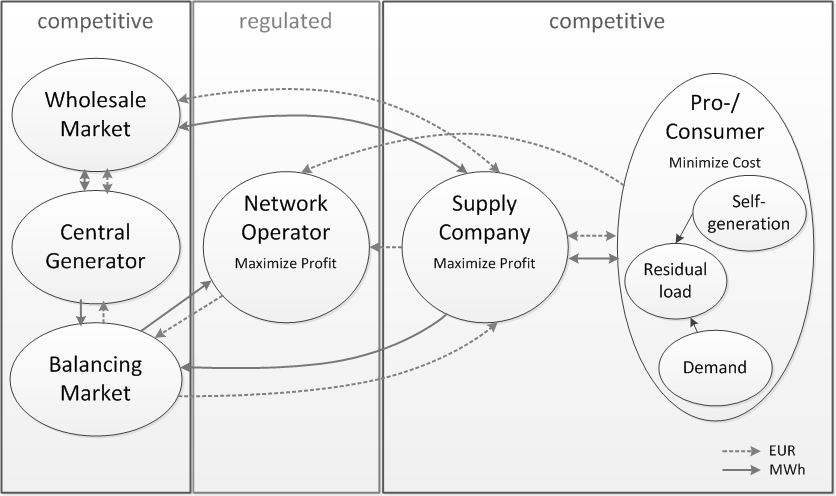
\includegraphics[width=85mm]{figures/market_structure.png}
  \caption{Simplified Illustration of the Structure of Energy Retail
    Market}
  \label{fig:market_structure}
\end{figure}

\subsection{Methodology}
\label{sec:econ-2}
In most cases, novel cooperative control strategies require clearly
defined business models. Here, it has to be specified, which market
participants are involved and how their role and responsibilities in
these new business models are allocated. It has to be described, which
technology portfolio is considered in the business model and which
technologies are controlled by the control strategy in which
way. Furthermore, it is important to clearly define the ownership of
the technology portfolio - in some cases leasing models may be
considered - and to decide who operates the controller. In addition,
if the controller reacts on price signals, the tariff design has to be
specified. Considered tariff types comprise flat tariffs, time-of-use
tariffs (TOU), real-time-pricing (RTP), two-part tariffs and
peak-load-pricing. 

Once the control strategy and the corresponding business model are
clearly defined, an economic trade-off analysis in comparison with the
status quo has to be conducted. In order to fulfill the cooperative
concept, a  crucial condition here is a Pareto-criterion. This
requires that no market participant has higher cost or lower profit –
depending on the respective objective – with the new business model
than with the status quo. Thus, the formal framework for economic
modelling consists of individual optimization problems for all
involved market participants. 

\subsection{Economic Models}
\label{sec:econ-3}
Since different hybrid control strategies and business models for
different market participants are analyzed, the economic models have
to be capable of considering various technology portfolios, several
tariff designs and multiple energy domains. To incorporate the hybrid
point-of-view, all quantities $\mathbf{q}$ and prices $\mathbf{p}$ are written as
three-dimensional vectors,
\begin{equation*}
  \mathbf{q}=(q^E, q^G, q^H )^T , \mathbf{p}=(p^E, p^G, p^H )^T , 
\end{equation*}
with each component representing another energy domain: electricity,
gas and heat. Depending on the research question, control strategy and
business model, the optimization problems have different time periods,
time resolutions and are either formulated as LPs or MILPs, if
investment decisions are considered. In the following, the considered
time period in years is written as $N$, the number of time steps per
year is denoted by $n$ and $k$ is the personal interest rate of each
market participant. 

\subsubsection{Customers}
To minimize their cost for meeting their energy demand, customers
generally have several possibilities. They can either procure all the
energy from a supply company via the energy distribution networks at a
certain tariff or they can invest in different technologies for energy
self-generation, conversion and storing. In addition they can also
invest in energy efficiency measures, like e.g. wall insulation, to
reduce their demand. If the demand of a standard passive customer is
denoted by $\mathbf{d}$, and the tariff by $\mathbf{p}$, then the cost is given by 
\begin{equation*}
  C = \sum_{y=1}^{N}(1+r)^{-y} \cdot \sum_{t=1}^{n} \mathbf{p}(y,t)^{T} \cdot \mathbf{d}(y,t)
\end{equation*}

If a prosumer is considered, this cost function can be gradually
extended to an optimization model by adding new terms and constraints,
describing additional technologies. Consider, e.g., a customer with a
heat pump and let the energy input vector of the heat pump be denoted
by $\mathbf{q}_{in}^{HP}$, the output by $\mathbf{q}_{out}^{HP}$ and the matrix,
describing the coefficient of performance, $\mathbf{COP}^{HP}$. Furthermore,
$\mathbf{q}$ describes the energy purchased from a supply company and the
investment cost of the heat pump are given by $I^{HP}$. Then the
optimization problem of this customer can be written as: 
%\begin{align*}
%  & \min & \sum_{y=1}^{N}(1+r)^{-y} \cdot \sum_{t=1}^{n} \mathbf{p}(y,t)^T &\cdot
%  \mathbf{q}(y,t) - I^{HP}, \\
%  & \textrm{s.t.}  & \mathbf{q}(y,t) + \mathbf{q}_{out}^{HP} (y,t)&  = \mathbf{d}(y,t) +
%                     \mathbf{q}_{in}^{HP} (y,t), \\
%  & & \mathbf{q}_{out}^{HP}(y,t) & = \mathbf{COP}^{HP} \cdot \mathbf{q}_{in}^{HP} (y,t), \\
%  & & \mathbf{q}(y,t), \mathbf{q}_{out}^{HP}(y,t), \mathbf{q}_{in}^{HP}(y,t) & \geq 0.
%\end{align*} % TODO? make a better align?
\begin{align*}
  & \min \sum_{y=1}^{N}(1+r)^{-y} \cdot \sum_{t=1}^{n} \mathbf{p}(y,t)^T \cdot
  \mathbf{q}(y,t) - I^{HP}, \\
  & \textrm{s.t. } \mathbf{q}(y,t) + \mathbf{q}_{out}^{HP} (y,t)  = \mathbf{d}(y,t) +
                     \mathbf{q}_{in}^{HP} (y,t), \\
  & \phantom{\textrm{s.t. }}\mathbf{q}_{out}^{HP}(y,t) = \mathbf{COP}^{HP} \cdot \mathbf{q}_{in}^{HP} (y,t), \\
  & \phantom{\textrm{s.t. }}\mathbf{q}(y,t), \mathbf{q}_{out}^{HP}(y,t), \mathbf{q}_{in}^{HP}(y,t) \geq 0.
\end{align*} % TODO? make a better align? Does this look better?
In a similar way other energy conversion technologies as well as
energy generation and storage systems can be added to the model. 

The customer tariff consists of three parts, namely, (i) the energy
tariff, which is paid to the supply company, (ii) network charges,
which are paid to the distribution system operator, and (iii) fees and
taxes. Each of these parts, in general, can have several components:
(i) a one-time initial payment or connection cost, (ii) an annual lump
sum, (iii) a quantitative component, which can be flat, TOU or RTP,
and (iv) a peak-load-pricing component; In order to incorporate these
different tariff types in the models, various objective terms and
constraints have to be added, which will not be further elaborated
here. 

\subsubsection{Supply Companies}
The supply company model has a very similar structure to the customer
model. The objective is given by the firm’s profit. The revenue is
determined by the quantities, retailed to the customers, multiplied by
the tariff, set in the business model design, and possible sales on
wholesale markets multiplied by the respective market prices. The
total cost consists of the investment cost and operational cost for
generation plants, coupling technologies and energy storage
devices. Additionally, if the supply company is buying energy from
wholesale markets or via long-term contracts, these expenses have to
be considered. If the purchased energy is transmitted via a network
and if it is used by a device at the supply company’s site, e.g. a CHP
fired by gas, network charges have to be paid as well. Otherwise, the
network charges are applied to the customers, consuming the energy. 

Furthermore, supply companies have to predict their generation and
their customers’ demand and report the respective schedules to a
clearing and settlement agency. If balancing energy is required to
uphold smooth network operation, they have to pay a share of the
resulting cost ex post, based on their deviations from the announced
schedule. 

Though the models for customers and supply companies, presented here,
are strictly cost-optimizing, they are adapted to match the operation
mode of the respective control strategy for business model
evaluation. 

\subsubsection{Distribution System Operators}
It has already been mentioned that DSOs are regulated. Within the
regulatory constraints, however, they try to maximize their
profit. Their revenue is given by the network charges of their
customers, also including supply companies, and their cost consist of
investment cost and operational (maintenance) cost for the network
components. The DSO model is formulated as a mixed-integer
investment-planning problem, where the annual decision options
comprise reinvesting, repairing or doing nothing per component. The
realized choices affect the expected failure rate, the cost and the
total asset value, which could be subject to regulatory constraints. 

Different regulatory frameworks provide incentives for different
investment and maintenance strategies. Price-cap or revenue-cap
regulations limit the annual revenue and typically facilitate
under-investments. Cost-of-service or rate-of-return regulations, on
the other hand, limit the profit by a percentage of the investments
and, thus, rather promote over-investments.

\section{Co-operative Control Strategy as 
Optimization over Planning Horizon}
\label{sec:control}

% scope of control strategy, 
The scope of hybrid-grid control strategy includes all major elements
of the participating grids. Note that, this not only includes grid
coupling devices such as CHP or heat-pump, but also includes
traditional elements such as fuel-based boilers or fuel-based
generators. The control also needs to optimize market side decisions 
(e.g. when to generate electricity and sell for CHP), and also needs
to provide signals for consumer side, too (when to store PV surplus
or feed-in).  

% our assumption on control: 
For our investigation, we model control strategy as one, central
module that can observe and signal all participating elements within
the hybrid-grid. This central module observes all the relevant
information over the hybrid-grid scope, and plans best co-operative,
co-beneficial decisions over the planning horizon. Essential
role of the co-operative control is to optimizes multiple grids
together to gain benefits that was not realized before from an
isolated single grid. 

\begin{figure}[th]
  \centering
  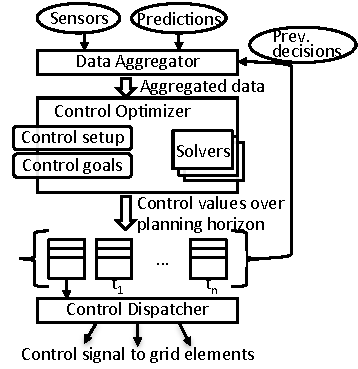
\includegraphics[width=50mm]{figures/control_flow.pdf}
  \caption{Control Flow}
  \label{fig:control}
\end{figure}

% description on data flow of control 
Figure \ref{fig:control} shows the conceptual data flow of the control
process. The flow starts with aggregated data. Data aggregator
collects various data sources over the ICT infrastructure such as
sensors, market prices, demand prediction data. The aggregator
provides a coherent data view over the participating grids. 

%mention ICT aspect?  
The collected data represent the status of the current grids as
observed by the control. They are fed into the control optimizer. The
control optimizer processes the data to derive best control
signals. The control has two pre-set parts. One is pre-defined model
of the hybrid-grid elements (control setup), and the other is the
target for optimization (control target). In turn, they form
constraints and objectives for the mathematical optimization, and
present the control problem as an optimization problem. To resolve
this optimization problem, the control module employs multiple solvers
(mathematical optimizers) to search and optimize control variables
over the problem space. This includes various mathematical programming
methods (linear programming, convex optimization, quadratic
programming) as well as heuristic optimization methods (such as
genetic algorithms). Once the solvers identify the best control
values, control module outputs the required control values for the
time horizon. This represents the current view of how the control
wants to control the grid elements. 

From the planned control values of the horizon, the current needed
control values are passed to grid elements as signals, by control
dispatcher. This optimization process is repeated in a planned time, 
since sensors and prediction data are updated. For our investigation,
we initially implemented the control to repeat planning for each 15
minutes. Horizon size is currently fixed as 24 hours. 

% differences to optimization of economical model 
Control strategy modeling is similar to actor modeling in economical
model, in the sense that it frames the problem within a optimization
framework. However, components in control model are generally far more
detailed, more numerous and complex (e.g. non-linear), since it
requires to check and provide control directions for actual devices
that works along the grid. Control's optimization behavior is 
heavily affected by technical constraints, such as keeping
load-factors of critical grid elements, and so on. Naturally the
control's problem space on the short-term, as optimize goals within
planning horizon, such as provide best-cost solution while satisfy
all technical constraints. This is not the case for economical model
which will focus on long-term  effects and long-term optimization
including adding / installing new devices. Economical model can do
this by simplify or ignoring technical constraints that are
successfully handled by control strategy. Thus, economical model
requires technical results from control-strategy evaluation to clarify
what can be projected within its model as technologically sound. 

% maybe a word about complexity? (linear is not enough?) 
% Also note that, due to model Linear models are no longer sufficient
% for control optimization,
% since various non-linear components are existing within control
% description. To cope with the heavy computational burden that can be
% caused by non-linear models, we employ various solvers in parallel
% and choose best output. 

\section{Holistic Investigation on the Impact of Hybrid Grid and
  Co-operative Control Strategy}  
\label{sec:hol} 

\subsection{Investigation process}

\begin{figure}[t]
  \centering
  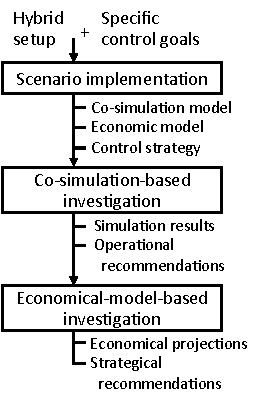
\includegraphics[width=40mm]{figures/holistic_flow.pdf}
  \caption{The flows of Holistic Investigation}
  \label{fig:flow}
\end{figure}

%[starting point, making a sceanrio: First step, hybrid setup +
%specific goal and coupling device. -> example, setup 1, ... setup 2,
%... ] 
\paragraph{Defining Scenario} 
The investigation starts from designing a specific hybrid evolution
scenario. In our context, a {\em scenario} means a hybrid setup
(Table \ref{tab:1})) instantiated into a concrete situation, bounded
by specific control goals and hybrid devices. For example, {\em
  Co-operative suppliers} setup of Skellefte\aa can be turned into a
scenario of ``better peak-boiler with hybrid strategy'', by adding
electric boilers in addition to existing CHP and oil-peak
boilers. Control goal for this scenario can be set as, a) best cost
peak-heat supply by tapping into fluctuating electricity price, and b)
reduce total green-house gases. This forms a concrete investigation
scenario that can be evaluated and compared with current
state-of-the-art. 
% ulm scenario also? maybe 

\paragraph{Scenario Implementation} 
Once a scenario is given, the first step of the investigation process
is {\em Scenario Implementation}. This includes building of
simulation models for the target site, implementing control model that
meets the control goal over the simulated grids, and the
implementation of economical model that can describe the major actors 
of the scenario. If we follow the example of ``better peak-boiler''
scenario, simulation models to be implemented are District heat grid
simulation and Power grid simulation of the target site in detail,
where the two simulations are ran coupled by a co-simulation
tool. A control model is implemented to control the simulated
components on the simulation; such as CHP, added electric boilers, oil
boilers, heat storage and power grid switches and so on. Economical
model incorporate all major contributors of the scenario, including
major devices (the above mentioned CHP and boilers, but not
on simulation level, but on their economical behaviors), and
stake-holders behavior (here the expected long-term behavior of power
and heat providers).  

\paragraph{Simulation-based Investigation} 
With the implementation done, the next step is {\em
  Co-simulation-based investigation}. This step is characterized by
many simulation runs for testing the control strategies, which are
instances of control models introduced in Section \ref{sec:control}. 
Each competing control strategy is being evaluated over the target
grids in various different, but relevant combination of situations. By
following the example of peak-boiler scenario, a set of control
strategy will be evaluated on all variations of demand conditions
(e.g. cold, not-so-cold winter), price  conditions (high/low price
ratio of oil to electricity), and various boiler sizes (adding single
to multiple power to electricity coupling device), etc. Simulation
investigation systemically covers all possible combinations.  

Note that, this simulation environment is a co-simulation
environment. In a co-simulation, each simulation (e.g. Heat grid
and Power grid simulation) works and exchange information at the same
time, bounded by a co-simulation tool. Detailed description on this
co-simulation environment is outside of the scope of this paper. For
our investigation, we use Power Factory as power grid simulation, and
Dymola for District Heat simulation, and FMI++ as the co-simulation
driver. Interested readers are kindly asked to refer to \cite{} for
co-simulation techniques and tools.   
% add references or footnote for PowerFactory, Dmola and FMI++? 

One direct result of the simulation investigation is all the values
that are observed and saved from a simulation run. The observed values
are processed further by technical evaluation measures, which can
evaluate and compare target hybrid control strategy with baseline. By
comparing evaluated results, investigators can draw meaningful
conclusions. We call the conclusions from
simulation results as ``Operational recommendation''.  
Operational recommendation includes the modeled control strategy
itself (the best control strategy among tested), and lessons learned
from simulation operation of the scenario.  
% For the peak-boiler scenario example, this is something like
%``24 hour prediction + electric boiler charging heat-storage" was the
% best control regardless of e-boiler size. With the strategy, and
% oil/power price condition of 2014, with single 24MW e-boiler, leads 
% 99\% reduction of oil-usage and green house gases from oil. But
% coldest winter like 2010, oil boiler operations are still expected
% with 15% of peak-load.  

\paragraph{Investigation with Economic-model}

Final step of the investigation is {\em 
Simulation-based investigation alone, cannot answer many important
questions of 


[what economical model investigation does] 

[why this step is required as separate step] 


%% Gil: I am not so sure visiting KPI names/content in detail is
%% meaningful --- given the space. (==> No KPI section for now.) 

% \subsection{Evaluation Measures}
% \label{sec:kpi}
% Table \ref{table:kpi} summarizes the key performance indicators
% (KPIs), that we have adopted after analyzing requirements introduced 
% in Section \ref{sec:req-2}. 

% \begin{table}[t]
%   \centering
%   \caption{Key Performance Indicators}
%   \label{table:kpi}
%   \begin{tabular}{|p{3.8cm}|p{3.8cm}|}
% \hline
%   Technical Indicators: Heat Grid &  \\ \hline
%   Technical Indicators: Power Grid & \\ \hline 
%   Economic and Social Indicators & \\ \hline 
%   \end{tabular}
% \end{table}

% % Electricity grid 
% % 1) Utilization of grid elements (loading of grid components)
% % 2) voltage quality performance 
% % 3) level of losses in transmission / distribution 
% % 4) Hosting capacity for distributed energy resources 

% % Heat grid 
% % 1) Base heat load factor 
% % 2) Maximum heat load production 
% % 3) Peak oil boiler load factor 
% % 4) Heat distribution losses 

% % Eco/Social 
% % 1) Reduction of total/specific system cost 
% % 2) Fulfillment of Pareto-criterion 
% % 3) (Internal) Rate of Return of Investments 
% % 4) Effectiveness and Efficiency of financial support 
% % 5) Energy savings 
% % 6) Fossil Fuel Savings 
% % 7) Reduction of Greenhouse gas emissions 
% % 8) Security of Supply 

% % [about one-two paragraphs on the KPIs as whole???] 

\section{Outlook and Conclusion}
\label{sec:con} 
Currently there are two investigations on-going, one for each test
site. For Skelleftea, the first scenario is about phasing out peak oil
boilers of district heat grid, in a manner both economically and
environmentally beneficial. For operational recommendation, we expect
optimal size and type of boiler, best co-operative control strategy
over two grids, cost and greenhouse gas footprints of the optimal
control. For strategical recommendation, the economical model will
give us 20-years view of cost and investment analysis, with respect to
various range of possible future fuel / electricity price changes.  

For Ulm site, the first investigation is about ''store surplus PV as
heat in house-hold'', where the control goal is minimize MV feed-in,
and minimize loads over critical grid elements. Operational analysis
will give us the result of various heating devices (e-boiler, heat
pump), control strategy over the set of devices, with their impacts on
storing PV surplus power. Economical analysis will tell us on what
condition this strategies will make sense --- such as adoption of new
feed-in tarif, cost analysis and comparison to alternatives such as
network upgrade, and also cost / gain projections over long-term such
as 20 years.  

There are also plans for more advanced hybrid investigations; such as
what would be the ideal heat/power co-supply in Skelleftea for
the expected 20\% more population in 2030, how to take benefit of 
hybridization with demand side management, and investigation of new
business chances in Ulm site with new hybrid-district heat grid, and
so on.    

The proposed two-step investigation process of the paper enables us to 
have concrete, thorough and realistic checks for each scenario that
we look into. The completeness comes from the ability to check and
sample details on both operational (short-term, technical) and
strategical (long-term,  economical and social) aspects of the given
setup and scenario. We believe that this enable us to form a holistic
recommendation for stake-holders of each investigation, and we also
believe that the holistic recommendations will provide valuable
insights for the possible future energy grid evolution. 


% use section* for acknowledgment
%\section*{Acknowledgment}
% when we get accepted... I think. 

% trigger a \newpage just before the given reference
% number - used to balance the columns on the last page
% adjust value as needed - may need to be readjusted if
% the document is modified later
%\IEEEtriggeratref{8}
% The "triggered" command can be changed if desired:
%\IEEEtriggercmd{\enlargethispage{-5in}}

% references section

\bibliographystyle{plain}
\bibliography{Orpheus_ISGT-EUR.bib}

\end{document}



\message{ !name(Orpheus_ISGT-EUR.tex) !offset(-874) }
